\documentclass[a4paper,ngerman]{scrartcl}

\usepackage{amsmath}
\usepackage{amsfonts}
\usepackage{amssymb}
\usepackage[utf8]{inputenc}
\usepackage{graphicx}
\usepackage[ngerman]{babel}
\usepackage{hyperref}
\usepackage{float}
\usepackage{caption}
\usepackage{subcaption}
\usepackage{multirow}  %for tables
\usepackage{icomma} % Handle german comma as decimal point in numbers
\usepackage{units,siunitx} % Write units with correct spacing
\usepackage{upgreek} % provide non-italic greek letters
\usepackage{url}
%\usepackage{subfig}

% Formatting of table & figure captions
\captionsetup{font={sf,footnotesize},labelfont=bf,skip=6pt}
\captionsetup[sub]{font={sf,footnotesize}} % setting for subcaptions
\sisetup{ locale = DE, % use "," as decimal point instead of "."
per-mode=fraction, % use fractions instead of ^{-1} when doing \si{... \per ...} 
exponent-product={\cdot},% used \cdot in front of 10^x
separate-uncertainty % give out uncertainty with \pm instead of in brackets
}  
\setlength{\abovecaptionskip}{6pt}
\setlength{\belowcaptionskip}{0pt}

\title{Landé-Faktor des Myons\\Versuchsvorbereitung}
\date{\today}
\author{Michel Rausch, Michael Eliachevitch}

\begin{document}

\maketitle
\tableofcontents
\newpage

\section{Einleitung}
\label{sec:einfuhrung}
% Ziel: Bestimmung der Lebensdauer und des Landé-Faktors von Myonen, 
% Myonen sinde Sekundärteilchen der kosmischen Strahlung
% wir werden ständig mit Myonen bombardiert, ohne es zu merken


\section{Theoretische Grundlagen}
\label{sec:theorie}

\subsection{Enstehung von Myonen in Luftschauern}
\label{sec:luftschauer}

Atmosphärische Myonen entstehen beim Auftreffen von hochenergetischen kosmischen Strahlen auf die Erdatmosphäre.


\begin{figure}[tbh!]
  \centering
  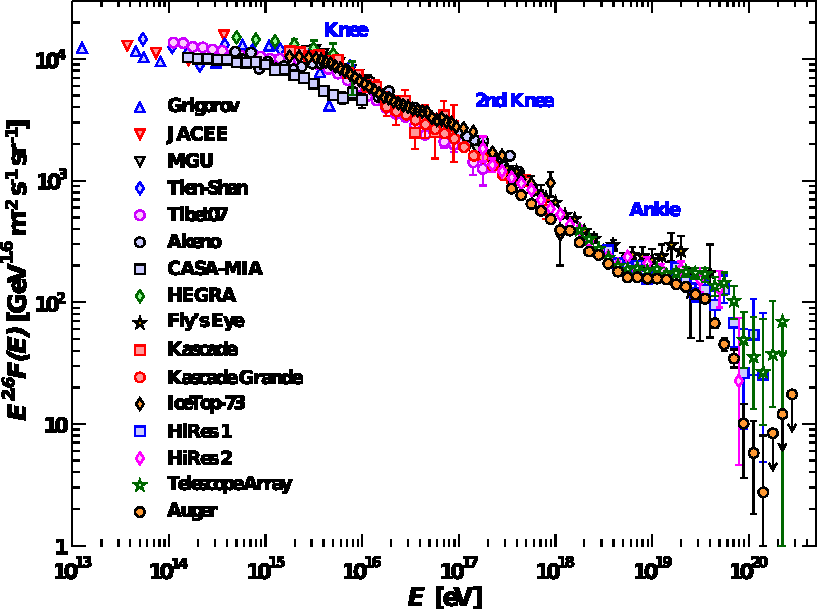
\includegraphics[width=0.8\textwidth]{abbildungen/cr_spectrum_pdg14.pdf}
  \caption{\textbf{Spektrum der kosmischen Strahlung für alle Teilchen aus den Daten von verschiedenen Luftschauerexperimenten.} Aufgetragen ist der differentielle Fluss, gewichtet mit der Energie $E^{2.6}$, gegen die Teilchenenergie pro Nukleon. Gut zu sehen sind das Knie bei etwa $\SI{e15}{eV}$ und der Knöchel ab $\SI{e19}{eV}$, was die beiden Punkte sind, bei denen sich der Faktor $\Gamma$ des Potenzspektrums der kosmischen Strahlung ändert. Mit den neusten experimentellen Daten scheint es auch einen zweiten Knöchel bei $\SI{e17}{eV}$ zu geben. Stand 2014 \ref{ref:pdg14}.}
  \label{fig:cr_spectrum}
\end{figure}
% kurz schreiben, dass hochenergetische kosmische teilchen luftschauer erzeugen,
% bei denen durch hadronische wechselwirkungen geladene pionen entstehen, bei deren zerfall myonen entstehen
% vielleicht auch weglassen und erst später beim kapitel zum spin
% lebensdauer von myonen
% evtl. grober wert für den fluss von myonen aus luftschauern


\subsection{Abbremsung von Myonen in Materie}
\label{sec:wwmitmaterie}
% bei sehr hohen energien (> 1 TeV) bremmstrahlung
% bei energien im GeV Bereich Ionisation (Myonen sind 'mips' -> kleiner wirkungsquerschnitt)
% wechselwirkungen mit atomen bei niedrigen energien: 
% niederenergetische myonen wie elektronen in kern gebunden -> schneller zerfall
% antimyonen bilden kernähnliche struktur durch elektroneneinfang -> myonium

\subsection{Polarisation von Myonen}
\label{sec:polarisation}
% schwacher wechselwirkung -> vektorielle kraft und paritätsverletzung
% d.h. masselose teilchen immer linkshändig, antiteilchen rechtshändig
% da pion spin 0 hat und neutrino linkshändig ist, muss positron/antimyon auch linkshändig sein
% wegen schwacher ww wären positronen und antimyonen "lieber" rechtshändig
% da positronen kleinere masse haben als anti-muonen (faktor ~200), ist bei ihnen die rechtshändige komponente stärker unterdrückt
% analog für antineutrinos und elektronen/myuonen
% daher zerfall von piplus/piminus hauptsächlich in muonen und nicht in elektronen/positronen

% zerfall in vorwärts und rückwärtsrichtung
% myon erhält dadurch in vorwärts und rückwärtsrichtung unterschiedliche energien im laborsystem bei gleichen pionenenergien
% unterscheidbar durch polarisation



\subsection{Nachweis des Myonenzerfalls}
\label{sec:nachweis}

% die theorie hiervon kann ich auch noch nicht gut (michael)
% aber müsste nicht viel sein

\subsection{Präzission von Myonen im Magnetfeld}
\label{sec:prazission}
% gyromagnetische verhältnis gamma, landé-faktor g erklären
% präzission im magnetfeld
% am wichtigsten ist eigentlich nur folgende gleichung:
\begin{equation}
g = \frac{\gamma \hbar}{\mu_\mathrm{B}} = \frac{\hbar \omega}{\mu_\mathrm{B}\mathrm{B}}
\end{equation}

\subsection{Messprinzip}
\label{sec:messprinzip}
% zerfall von myonen erfolgt exponentialgesetz
% wie misst man präzission?
% -> angelegtes magnetfeld
% formeln...
\clearpage

\section{Versuchsaufbau und Durchführung}
% von oben nach unten: Szinti 1, Szinti 2, Kupferabsorber in Magnetfeld, Szinti 3
% Koinzindenz und Veto-Schaltung erklären: 
% D.h. Wir nehmen nur die Ereignisse, wo 1 und 2 gleichzeitig ausschlagen (Koinzindenz) und 3 NICHT ausschlägt (Veto bzw Antikoinzindenz)
% erklären was ein diskriminator in der analog-digitalwandlung ist und wie die schwelle (trigger) eingestellt werden muss:
% trigger muss so sein, dass untergrund unterdrückt wird und man nur hauptsignal sieht
% zu hoher trigger verringer unnötig statistik
% trigger für veto (szinti 3) lieber etwas niedriger als zu hoch, damit man keine falschen ereignisse aufnimmt
% was ist ein TAC (zeit-amplituden-converter) und zeiteichung ?


\begin{figure}[tb!]
  \centering
  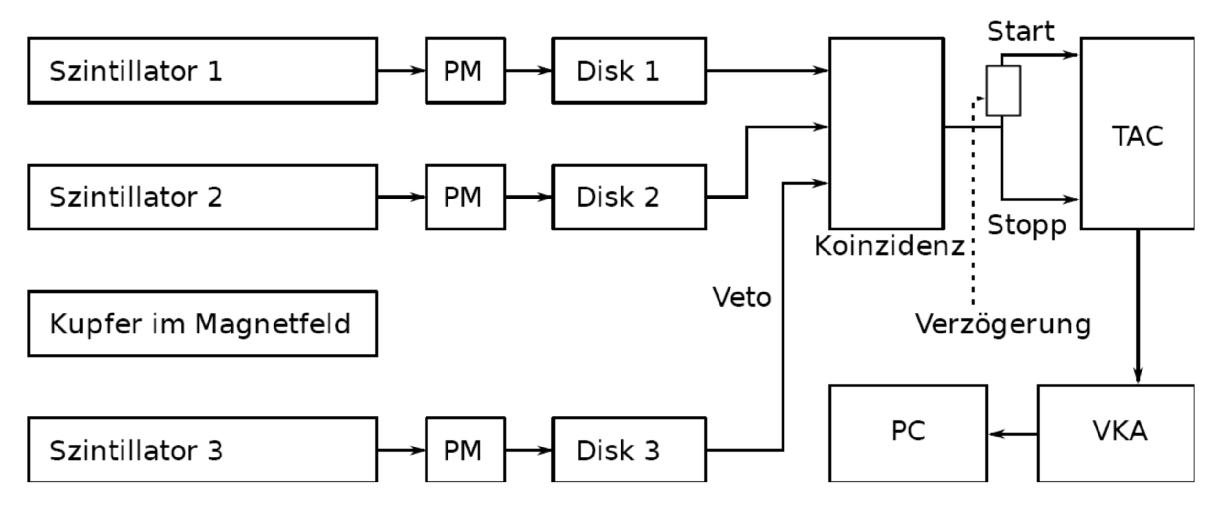
\includegraphics[width=0.8\textwidth]{abbildungen/aufbau_skizze.png}
  \caption{\textbf{Skizze des Versuchsaufbaus.} 
  \\ 
  Drei Kunstoffszintillatoren und eine Kupferplatte mit einer Dicke von jeweils $\SI{2}{cm}$ sind übereinander angeordnet. 	Das Signal aus den Szintillatoren wird mit Photomultpliern (\textbf{PM}) verstärkt. Bei den definierten Signatur $1 + 2 + \overline{3}$ wird von der Koinzidenz ein Signal für den Start, bzw. Stopp der Messung gegeben. Das Startsignal wird um einige Nanosekunden verzögert, damit der Time to Amplitude Converter (\textbf{TAC}) das Signal verarbeiten kann. Über einen Vielkanalanalysator (\textbf{VKA}) wird das Signal an einem Rechner (\textbf{PC}) analysiert.
  \\Quelle: [\ref{ref:bb}]}
  \label{fig:blmaufbau}
\end{figure}




\clearpage
\section{Quellen}
\begin{enumerate}
\item \emph{Einführung in das Kernphysikalische Praktikum} von F. K. Schmidt, 
  Überarbeitung von J. Wolf, Ausgabe September 2009. \label{ref:bb}
\item K.A. Olive et al. (Particle Data Group), Chin. Phys. C, 38, 090001 (2014). \label{ref:pdg14}
\end{enumerate}



\end{document}
